%各自の環境に応じて修正
%\documentclass[a4paper,11pt]{jarticle}
\documentclass{ltjsarticle}

\usepackage{enumitem}
\usepackage{appendix}
\usepackage{float}
\usepackage{bm}
\usepackage[dvipdfmx]{graphicx}
\usepackage[dvipdfmx]{color}
\usepackage{tikz}
\usepackage[T1]{fontenc}
\usepackage[utf8]{inputenc}
\usepackage{lmodern}
\usepackage[american]{babel}
\usepackage{subcaption}
\usepackage{tabularx}
\usepackage{graphics}
\usepackage{physics}
\usepackage{mathtools}
\usepackage{amssymb,amsmath,amsfonts,eurosym,geometry,graphicx,caption,color,setspace,comment,footmisc,caption,pdflscape,array,hyperref}
\usepackage{booktabs}
\usepackage{siunitx}
\newcolumntype{d}{S[
    input-open-uncertainty=,
    input-close-uncertainty=,
    parse-numbers = false,
    table-align-text-pre=false,
    table-align-text-post=false
]}
\usepackage{listings} 
\usepackage{xcolor}
\lstdefinestyle{matlab}{
  language=Matlab,
  basicstyle=\ttfamily\footnotesize,
  keywordstyle=\color{blue},
  stringstyle=\color{red},
  commentstyle=\color{green!60!black},
  numbers=left,
  numberstyle=\tiny\color{gray},
  stepnumber=1,
  frame=single,
  breaklines=true,
  showstringspaces=false
}

 
\usepackage{titlesec}
\titleformat*{\section}{\Large\rmfamily}
\titleformat*{\subsection}{\large\rmfamily}
\titleformat*{\subsubsection}{\rmfamily}
 

%テキストの表示領域の調節
\setlength{\textwidth}{\paperwidth}
\addtolength{\textwidth}{-40truemm}
\setlength{\textheight}{\paperheight}
\addtolength{\textheight}{-45truemm}

%余白の調節
\setlength{\topmargin}{-10.4truemm}
\setlength{\evensidemargin}{-5.4truemm}
\setlength{\oddsidemargin}{-5.4truemm}
\setlength{\headheight}{17pt}
\setlength{\headsep}{10mm}
\addtolength{\headsep}{-17pt}
\setlength{\footskip}{5mm}

% \renewcommand{\thesection}{\Alph{section}}
% \renewcommand{\thesubsection}{\alph{subsection}}


\title{Macroeconomics $\mathrm{II}$ Homework 3}
\date{\today}
\author{Graduate School of Economics, The University of Tokyo\\[4mm]29--246029 Rin NITTA\\ 29-246033 Rei HANARI \\ 29--246004 Kosuke IGARASHI}

\begin{document}
\maketitle

\section*{Q1}
\subsection*{(a)}
A recursive problem of household is the Bellman equation with an offer $w$ in hand as below.\\
Let $v(w)$ denote the reservation wage.

\begin{gather*}
  v(w) = \max_{accept, reject} \left\{ \frac{w}{1 - \beta}, c + \beta \int^B_0 v(w')dF(w') \right\} 
\end{gather*}

\subsection*{(b)}
Let $\bar{w}$ denote the reservation wage.
\begin{align*}
    v(w) = 
    \begin{cases}
      \max_{accept, reject} \{ \frac{w}{1 - \beta}, c + \beta \int^B_0 v(w')dF(w') \} & \text{if } w \leq \bar{w}  \\
      \frac{w}{1 - \beta} & \text{if } w \geq \bar{w}
    \end{cases}
\end{align*}

Now,
\begin{align*}
    v(\bar{w}) = \frac{\bar{w}}{1 - \beta} = c + \beta \int_0^{\bar{w}} 
 \frac{\bar{w}}{1 - \beta} dF(w') + \beta \int^B_{\bar{w}} \frac{w'}{1 - \beta} dF(w')
\end{align*}
Then, we get $\bar{w} - c = \frac{\beta}{1 - \beta} \int^B_{\bar{w}} (w' - w)dF(w')$.\\
Define the RHS as
\begin{align*}
    h(w) = \frac{\beta}{1 - \beta} \int^B_{\bar{w}} (w' - w) dF(w')
\end{align*}
Note that
\begin{align*}
    &h(0) = E[w] \frac{\beta}{1 - \beta}\\
    &h(B) = 0\\
    &h'(w) = \frac{\beta}{1 - \beta} [ -(w' - w) f(w) + \int^\beta_w (-1) dF(w') ] = - \frac{\beta}{1 - \beta} [1 - F(w)] < 0\\
    & h''(w) = \frac{\beta}{1 - \beta} F'(w) > 0
\end{align*}
So the relationship between cost and benefit is described as below.\\
\begin{figure}
    \centering
    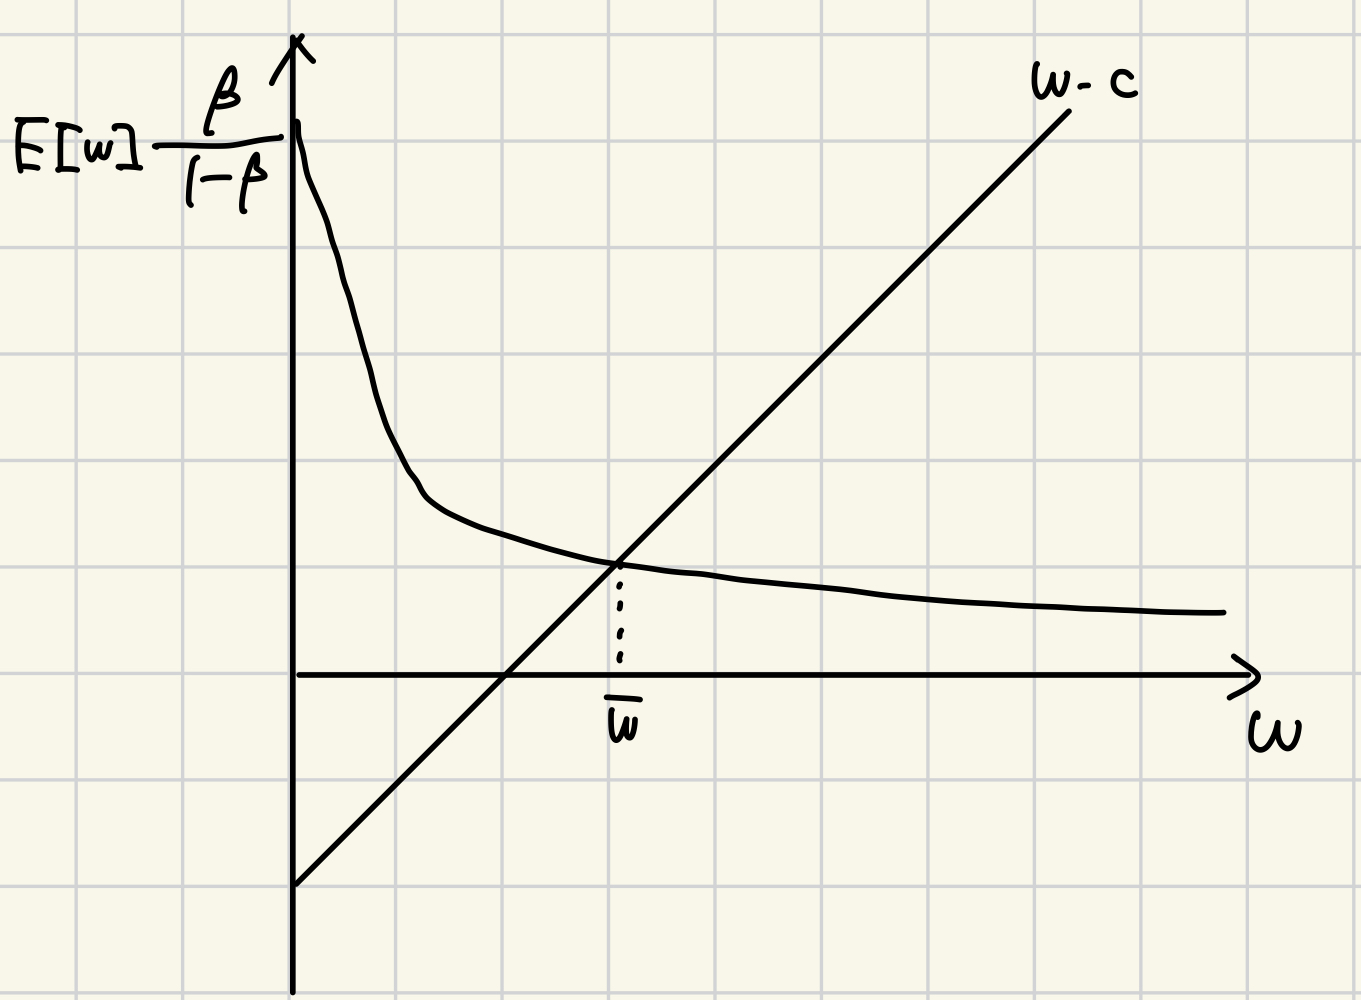
\includegraphics[width=0.5\linewidth]{hw3_1_graph.jpg}
    \caption{Relationship between cost and benefit}
    \label{fig:enter-label}
\end{figure}
Therefore, a rise in $\beta$ leads to a rise in $\bar{w}$.\\
An increase in $\beta$ means that people become more patient, valuing future benefits more highly and thus aspiring to wait for higher wages.\\
This aligns with the results derived from the equation.

\subsection*{(c)}
From the graph, a rise in $c$ leads to a rise in $\bar{w}$.\\
An increase in $c$ means that the compensation for rejecting an offer increases, leading job seekers to pursue employment with higher offers. This is consistentwith the results derived from the equation.


\section*{Q2}
Let the consider the value function for employed and unemployed workers.\\
Let $\bar{w}$ denote the reservation wage.\\
(i) Employed workers:\\
The budget constraint of an unemployed worker at time $t$ is
\begin{align*}
    a_{t+1} \leq R_t(a_t + w_tn_t - c_t)
\end{align*}
When this constraint binds, $c_t = a_t + w_tn_t - \frac{a_{t+1}}{R_t}$.\\
So the value function is
\begin{align*}
    v(w) = \max_{n_t} \{ p(a_t + w_tn_t - \frac{a_{t+1}}{R_t}, 1 - n_t) + \beta\int_R v(w)dH(R) \}
\end{align*}
(ii) Unemployed Workers:\\
The budget constraint of an unemployed worker at time $t$ is
\begin{align*}
    a_{t+1} \leq R_t(a_t + z - c_t)
\end{align*}
When this constraint binds, $c_t = a_t + z - \frac{a_{t+1}}{R_t}$.\\
So the value function is
\begin{align*}
    v(w) = \max_{n_t} \{ z + \beta \int^B_0 \int_R v(w') dF(w) dH(R) \}
\end{align*}


\section*{Q3}

\section*{Q4}

\subsection*{(a)}

Vacancies are filled at rate
\begin{gather*}
  \frac{m(u,v)}{v} = \frac{u}{v+u} = \frac{\frac{1}{\theta}}{1+\frac{1}{\theta}} = m \left(\frac{1}{\theta}, 1\right) \equiv q(\theta)
\end{gather*}
As we did in the lecture, suppose there is a continuum of workers with measure 1. Every period, $\lambda(1-u)$ workers enter unemployment, and $\theta q(\theta) u $ workers find a job.
\begin{gather*}
  \Delta u = \lambda(1-u) + \theta q(\theta) u
\end{gather*}
At the steady state, $\Delta u = 0$, so we have
\begin{align*}
  u 
  &= \frac{\lambda}{\lambda + \theta q(\theta)}\\
  &= \frac{\lambda}{\lambda + \frac{1}{1+\frac{1}{\theta}}}\\
  &= \frac{\lambda}{\lambda + \frac{\theta}{\theta+1}}
\end{align*}

\subsection*{(b)}
At any period of steady state, $1-u$ workers are employed. For each employed worker, the probability of transitioning from employment to unemployment is $\lambda$, and the probability of being unemployed for $n$ periods is $(1- \theta q(\theta))^n$. Therefore, for each $n=1,2,\cdots$, 
\begin{gather*}
  u_n = \lambda (1-u) (1- \theta q(\theta))^n
\end{gather*}
\begin{align*}
  \sum_{n=1}^{\infty} u_n
  &= \frac{\lambda (1-u)}{1 - (1- \theta q(\theta))}\\
  &= \frac{\lambda \left(1-\frac{\lambda}{\lambda + \frac{\theta}{\theta+1}}\right)}{\theta q(\theta)}\\
  &= \frac{\lambda}{\lambda + \frac{\theta}{\theta+1}}\\
  &= u
\end{align*}

\subsection*{(c)}

At each period, the government's total tax revenew is $(1-v)\tau$, and the government's total unemployment benefit is $u_1 z$, where $u_1$ is the number of workers who have been unemployed for 1 period. Then the government's budget constraint for each period is
\begin{gather*}
  (1-v)\tau = u_1 z
\end{gather*}

\subsection*{(d)}

\begin{align*}
  V &= -pc + \beta \{q(\theta)J + [1-q(\theta)]V \}\\
  J &= p - w + \beta[\lambda V + (1-\lambda)J]
\end{align*}

\subsection*{(e)}

Workers' states are classified in 3 states: employed, unemployed for 1 period, and unemployed for 2 or more periods. 
Let $U_1$ be the value of unemployment for 1 period, $U_2$ be the value of unemployment for 2 or more periods, and $W$ be the value of employment. Then,
\begin{align*}
  U_1 &= z + \beta \left\{ \theta q(\theta) W + [1-\theta q(\theta)] U_2 \right\}\\
  U_2 &= 0 + \beta \left\{ \theta q(\theta) W + [1-\theta q(\theta)] U_2 \right\}\\
  W &= w + \beta \left\{\lambda U_1 + (1-\lambda) W \right\}
\end{align*}

\subsection*{(f)}

Free entry implies $V=0$. Then, solving the equations in (d) gives
\begin{gather*}
  p = w + \frac{\left(\frac{1-\beta}{\beta} + \lambda\right)pc}{q(\theta)} =  w + \left(\frac{1-\beta}{\beta} + \lambda\right)pc (\theta+1)
\end{gather*}
Post vacancies up to the point where marginal product $p$ equals wage $w$ plus expected capitalizes value of hiring costs.

\end{document}